\section{Easily Reusing Existing Node/Link Mapping Algorithms}
The \texttt{SimpleDijkstraAlgorithm} is an example of how to implement an algorithm to solve the virtual network mapping, 
when the virtual link and node mapping are performed as a single stage. 
However, most of the algorithms to solve the VNE are divided in two stages:
\begin{enumerate}
	\item Virtual node mapping (performed in first place) and
	\item Virtual link mapping (performed in second place).
\end{enumerate}
To facilitate the task of implementing a VNE algorithm, the abstract \texttt{vnreal.algorithms. GenericMappingAlgorithm} class should be used.

The \texttt{GenericMappingAlgorithm} class takes two parameters: NodeMapping and LinkMapping. 
These need to be derived from the two classes \texttt{vnreal.\-algorithms.\ AbstractNodeMapping} and \texttt{vnreal.algorithms.AbstractLinkMapping}, respectively. 
In this way, the node mapping and link mapping stages can be implemented independently of each other. 
This has an important advantage: the node and link mapping stages of different algorithms can be combined, 
which may leads to different results.

GenericMappingAlgorithm works by processing each time a different virtual network 
request so the \textsl{getNext()} method returns a virtual network request. 
The \textsl{process(VirtualNetwork p)} method, 
receive this virtual network request and performs node mapping and link mapping stages. 
If at least one of them were not successful, 
all the mappings over that virtual network are undone and the method finishes 
(without realizing the mapping of that network); if they were both successful, 
the method finishes. 
The flow chart in figure \ref{fig:genericMappingAlgorithm} of the algorithm is shown next.
Different methods of \texttt{AbstractNodeMapping} and \texttt{AbstractLinkMapping} are described after the figure.
\begin{figure}[h]
  \begin{center}
		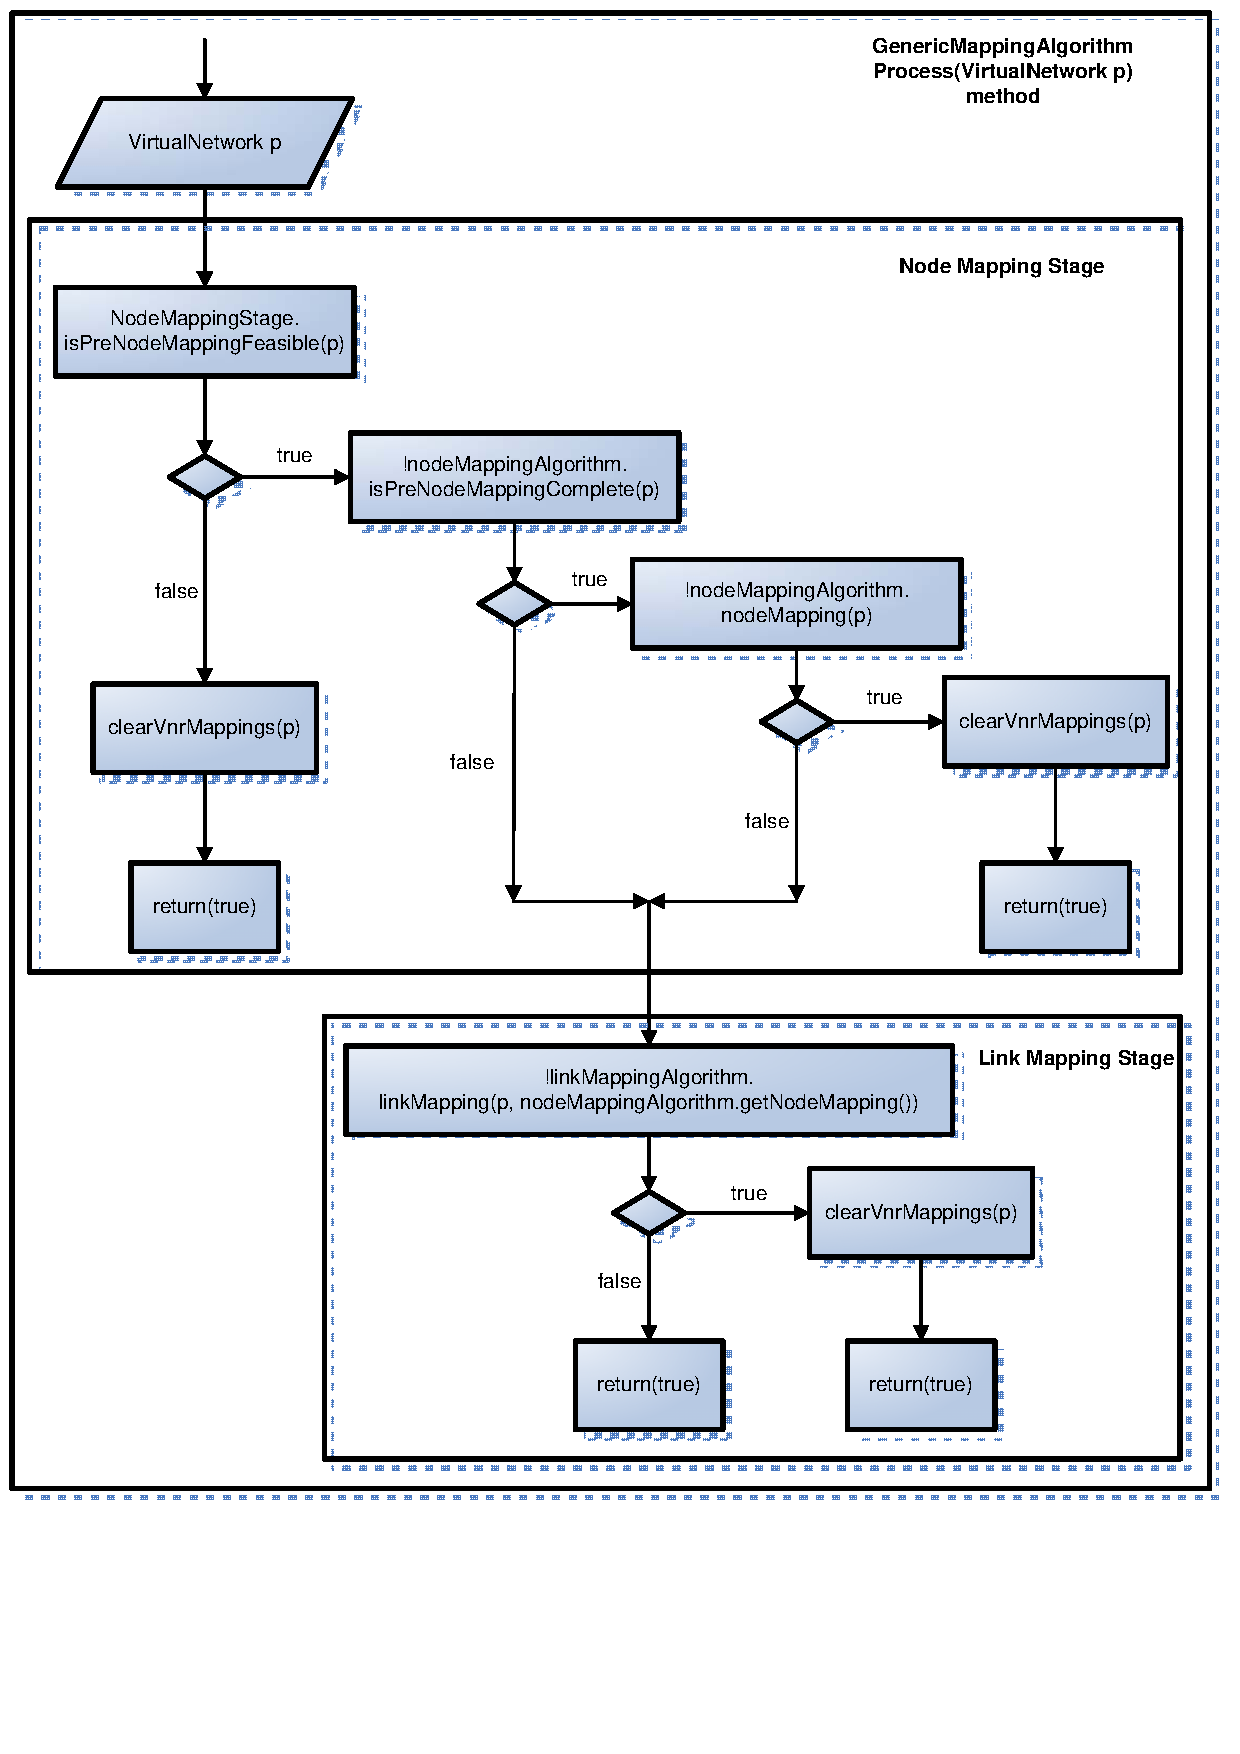
\includegraphics[width=\textwidth]{img/genericMappingAlgorithm.pdf}
	\end{center}
	\caption{Behaviour of \texttt{GenericMappingAlgorithm} }
	\label{fig:genericMappingAlgorithm}
\end{figure}

To implement a new algorithm that has both,
node and link mapping stage, two classes need to be implemented. 
Node mapping class that extends from \texttt{AbstractNodeMapping} and the link mapping class that extends from \texttt{AbstractLinkMapping}.


\subsection{AbstractNodeMapping}
Now let's check the \textbf{methods and variables} of \texttt{AbstractNodeMapping}:
\begin{lstlisting}
public abstract class AbstractNodeMapping {
	protected Map<VirtualNode, SubstrateNode> nodeMapping;
	private List<VirtualNode> unmappedvNodes;
	private List<SubstrateNode> unmappedsNodes;
	protected List<SubstrateNode> mappedsNodes;
\end{lstlisting}
The previous global variables have the following meaning:
\begin{itemize}
	\item \textsl{nodeMapping}: It is a list of Map type that contains the mapping of each \texttt{VirtualNode} 
	to its corresponding \texttt{SubstrateNode} after the node mapping is realized. 
	This variable should be updated while mapping is being performed.
	\item \textsl{unmappedvNodes}: It is a list with the virtual nodes that have not been mapped for the current virtual network request, after a predefined node mapping have been performed. ALEVIN supports the possiblity of predefining the mapping of a set of virtual nodes (possibly all) into its corresponding substrate nodes.
	\item \textsl{unmappedsNodes}: It is a list with the substrate nodes that have not been mapped, for the current virtual network request, after a predefined node mapping have been performed.
	\item \textsl{mappedsNodes}: It is a list with the substrate nodes that have been mapped, for the current virtual network request, performing the predefined node mapping.
\end{itemize}



\begin{lstlisting}
public boolean isPreNodeMappingFeasible(VirtualNetwork vNet)
\end{lstlisting}
ALEVIN supports a resource/demand called id in nodes: 
In this way it is possible to realize a predefined node mapping before the algorithm runs, it is enough to assign in the \texttt{IdDemand} of the virtual nodes the \texttt{IdResource} of the substrate nodes that are chosen to realize the mapping. 
The \textsl{isPreNodeMappingFeasible} method is responsible of realizing this predefined mapping and ensures that the resources of the mapped substrate nodes are enough to cover the demands of the virtual nodes. 
The method returns a false value if the mapping could not be performed. 
This method is already implemented in \texttt{AbstractNodeMapping} and used in \texttt{GenericMappingAlgorithm}. 
After the method is performed, \textsl{nodeMapping}, \textsl{unmappedvNodes}, \textsl{unmappedsNodes} and \textsl{mappedsNodes} are updated.



\begin{lstlisting}
public boolean isPreNodeMappingComplete() {
	return unmappedvNodes.isEmpty();
}
\end{lstlisting}
The method \textsl{isPreNodeMappingComplete()} checks if in the predefined node mapping stage the virtual node mapping has been performed completely or not. It is complete if all virtual nodes have been mapped, in this case no virtual node mapping should be performed. This method is already implemented in \texttt{AbstractNodeMapping} and used in \texttt{GenericMappingAlgorithm}.

\begin{lstlisting}
protected abstract boolean nodeMapping(VirtualNetwork vNet);
\end{lstlisting}
The \textsl{nodeMapping} method is the most important method of the class. 
\textbf{This method} is the one that has to be implemented in a new class (extending \texttt{AbstractNodeMapping}). 
It is important to know, when implementing this method, that probably a predefined mapping has been performed 
and some virtual nodes of the virtual network request have already been mapped (take into account \textsl{nodeMapping}, 
\textsl{unmappedvNodes}, \textsl{unmappedsNodes} and \textsl{mappedsNodes} variables). 
After the \textsl{nodeMapping} has been performed, the \textsl{nodeMapping} variable should be updated and the method should return a boolean value (true if the node mapping was successful, false otherwise).
To see some implementations of the \textsl{nodeMapping()} method, please go to \textit{vnreal.algorithms.nodemapping} package.




\subsection{AbstractLinkMapping}
Now let's check the \textbf{methods and variables} of \texttt{AbstractLinkMapping}:
\begin{lstlisting}
public abstract class AbstractLinkMapping {
	protected int processedLinks, mappedLinks;
\end{lstlisting}
The \texttt{AbstractLinkMapping} variables \textsl{processedLinks} and \textsl{mappedLinks} are used to update the progress bar of the algorithm. 
When a virtual link is being mapped, \textsl{processedLinks} should be incremented by 1, 
and when it have been already mapped, \textsl{mappedLinks} should also be incremented by 1.



\begin{lstlisting}
protected abstract boolean linkMapping(VirtualNetwork vNet,Map<VirtualNode, SubstrateNode> nodeMapping);
\end{lstlisting}
The main method of the \texttt{AbstractLinkMapping} class is the abstract \textsl{linkMapping} method. 
\textbf{This method} is the one that has to be implemented in a new class (extending \texttt{AbstractLinkMapping}). 
The input is the virtual network request and the already performed \textbf{node mapping}. 
The output of the method should be a boolean true if the node mapping was successful, false otherwise).


\subsection{Required GUI adoptions}
If you want your new algorithm to appear in the GUI, simply extend the class \texttt{vnreal. gui.menu.AlgorithmsMenu}.
